\documentclass[nofonts]{ctexart}
%\CTEXsetup[name={Step ,},number={\arabic{chapter}}]{chapter}
\setCJKmainfont[ItalicFont={AR PL UKai CN}]{AR PL UMing CN} %设置中文默认字体
\setCJKsansfont{WenQuanYi Micro Hei} %设置文泉驿正黑字体作为中文无衬线字体
\setCJKmonofont{WenQuanYi Micro Hei Mono} %设置文泉驿等宽正黑字体作为中文打字机字体

\usepackage{amsmath}
%\usepackage{wallpaper}
\usepackage{xcolor}
%\usepackage{pgf, tikz}
\usepackage{multirow}
\usepackage{listings}
\usepackage{color}

\definecolor{keywordcolor}{rgb}{0.8,0.1,0.5}
\definecolor{webgreen}{rgb}{0,.5,0}

%\usepackage[paperwidth=185mm,paperheight=260mm,text={148mm,210mm},left=21mm,includehead,vmarginratio=1:1]{geometry}
%\usepackage[raggedright]{titlesec}
%\titleformat{\chapter}[display]{\Huge\bfseries}{Step \,\thechapter\,}{1em}{}

%\usepackage{fancyhdr}
%\pagestyle{fancy}
%\fancyhf{}
%\fancyhead[ER, OR]{\leftmark}
%\fancyhead[EL, OL]{《编译实习》实习报告}
%\fancyfoot[C]{\thepage}
%\renewcommand{\chaptermark}[1]{\markboth{\thechapter.\ #1}{}}


\lstset{language=C,
basicstyle=\footnotesize,
keywordstyle=\color{keywordcolor}\bfseries, %\underbar,
identifierstyle=,
commentstyle=\color{green} \textit,
stringstyle=\color{red} \ttfamily,
showstringspaces=false,
frame=single,
numbers=left,
numberstyle=\tiny \color{blue},
backgroundcolor=\color{white},
captionpos=b
}


\begin{document}

\title{%
\vspace{-30mm}\Huge NachOS Lab4 实习报告 \vspace{10mm}}
\author{%
\Large 史杨勍惟 
\\[10mm] 1200012741 信息科学技术学院}
\date{2016,04,30}

\maketitle

\newpage
\tableofcontents
\newpage

\section{总体概述}
这次的Lab主要内容是虚拟内存上各种机制的实现,也是有史以来内容最多的一个 Lab。

\section{任务完成列表}
\begin{table}[h]
\footnotesize
\begin{tabular}{|c|c|c|c|c|c|}\hline
\textbf{Exercise 1} & \textbf{Exercise 2} &
\textbf{Exercise 3} & \textbf{Exercise 4} &
\textbf{Exercise 5} & \textbf{Exercise 6}\\\hline
Y & Y & Y & Y & Y & Y\\\hline

\end{tabular}
\begin{tabular}{|c|c|c|}\hline
\textbf{Exercise 7} & \textbf{Challenge 1} & \textbf{Challenge 2}\\\hline
Y & N & N\\\hline

\end{tabular}


\end{table}
\section{完成情况}
\subsection*{Exercise 1}
progtest.cc 中的 StartProcess 函数是启动用户程序的入口。从代码来看,StartProcess主要做了以下操作。
\begin{itemize}
\item 检查这是不是可执行文件;
\item 为其分配页表,初始化页表项;
\item 装入数据段、程序段;
\item 调用 machine->Run() 方法模拟用户程序在处理器上运行。
\end{itemize}

machine.cc 是对运行用户程序的硬件进行的模拟。这里我们发现,TLB在默认下是不开启的,需要通过宏定义开启。当TLB不开其的时候,Nachos使用PageTable,如果TLB开启,Nachos使用TLB。Machine类负责创建TLB。TLB的入口是RaiseException,当系统收到一种 Exception(例如 PageFault)时,此方法会被调用。从实现上来看,这也是我们要执行页面置换算法的入口。

translate.cc 定义了页表项和翻译规则。这里的页表项和我们在操作系统课上学到的一致。其翻译规则(虚拟地址到物理地址的转换规则)和我们操作系统课上学到的也类似。注意到,PageTable和TLB中的页表项结构是一样的。

\subsection*{Exercise 2 \& Exercise 3}

Exercise 2 的内容是捕获异常,我们只需在Exception类中中国添加一个新的Exception枚举体即可,这里我命名为TLBMissException。在ExceptionHandler中,加入一些条件判断,我们就可以确定异常类型是不是TLBMissException了。

随后就要对TLBMissException设计相应的异常处理函数,也就是设计页面置换算法。这里我选择了两种最简单也是最经典的页面置换算法,FIFO和LRU。

在具体实现上,我们需要设计两个函数TLBSwapFIFO和TLBSwapLRU,这两个函数首先计算出虚拟页号,通过索引得到页表项。然后在TLB中找有没有invalid的页表项,有的话就直接插入此处,没有的话,就需要选择一个页面置换。

\subsubsection*{FIFO}
对于FIFO算法,选择队头,所以用一个常量维护当前索引即可,算法如下:

\begin{lstlisting}
    int slot=TLBhead;
    TLBhead=(TLBhead+1)%TLBSize;
    int slot = 0;
    int min = tlb[0].comingTime;
    TranslationEntry *entry = NULL;		
    for(int i = 0; i< TLBSize;i++){     
        if(tlb[i].valid == FALSE){      //Found an empty TLB entry
	    slot = i;
           DEBUG('a',"Slot %d is empty.\n",slot);
	    break;
	}		
    }
    entry = &tlb[slot];

\end{lstlisting}

\subsubsection*{LRU}
对于LRU算法,需要为页表项维护一个上次访问时间的变量,一个比较直观的办法是把这个时间设成当时的totalTicks。实现过程只需要扫一遍TLB,选取最小值作为slot即可。
算法如下:
\begin{lstlisting}
    for(int i = 0; i< TLBSize;i++){     
        if(tlb[i].valid == FALSE){      //Found an empty TLB entry
	    slot = i;
           DEBUG('a',"Slot %d is empty.\n",slot);
	    break;
	}					    
       if(tlb[i].lastAccessTime < min){
	   min = tlb[i].lastAccessTime;
	   slot = i;
	 }
    }
    entry = &tlb[slot];

\end{lstlisting}

以下为FIFO测试结果:
\begin{figure}[h!]
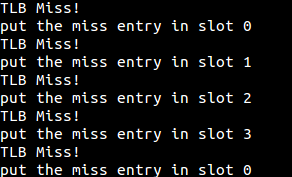
\includegraphics[width=2.5in]{fifo.png}
\end{figure}

以下为LRU测试结果:
\begin{figure}[h!]
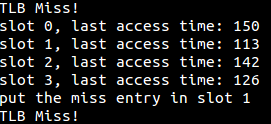
\includegraphics[width=2.5in]{lru.png}
\end{figure}

\subsubsection*{结果对比}
我把排序算法的数的个数射程了4,对比发现LRU的TLBMiss比FIFO少,对于排序算法来说这个结果是符合常理的。



\subsection*{Exercise 4}
我设计的数据结构是PageManager类,我的实现是基于位图的,而Nachos中的bitmap.cc提供了相关的接口。

以下是PageManager的接口:
\begin{lstlisting}
class PageManager
{
public:
	PageManager();
	~PageManager();
	int findPage();
	int numCleanPage();
	void markPage(int pagenum);
	void cleanPage(int pagenum);
private:
	BitMap *manager;
};
\end{lstlisting}

在实现过程中,首先需要在Initialize中初始化一个全局的PageManager对象,pageManager。在初始化过程中,我设定的位置大小为4096,即每个地址都是一个位。但是在分配的过程中还是基于页分配的,也就是每次以128位为一个单元分配。当然,这里本质上只需要$4096/128=32$个位就行了,但是4096本质上并不是一个大数字,所以我还是选择了每个地址映射到一个位。

为了简化Makefile的修改,我将PageManager类放到了machine.h和machine.cc中,而不是单独一个文件。


\subsection*{Exercise 5}
Nachos不支持多线程的本质在于虚拟内存的初始化过程中清零了整个物理内存。所以我修改了这个函数,只清零这个进程被分配的页号所对应的物理内存。

修改之后还是不支持多线程的运行的,我分析了很就,发现了Nachos不支持多线程的另一个原因。Nachos不支持多线程的另一个原因在于写入代码段和数据段的时候并不是按照页写的,这样就可能覆盖其他线程的代码段和数据段了,所以我们也需要修改这里。

测试过程中,我们需要模拟多线程运行。一种方法是如在命令行中添加多线程的执行方法,但是我觉得这种方法执行起来比较麻烦。我选择的在系统中模拟多线程,也就是在StartProcess函数中添加代码,模拟已有运行的一个用户程序。
我为sort测试例程建立一个新的地址空间,并且新建一个thread使得它的用户空间指向这个空间,然后,让新建立的线程Fork ,从而可以加入调度队列。在这个新进程的伊始,AddrSpace类的RestoreState()方法切换页表,然后调用 machine->Run() 执行。两个线程执行的都是sort程序。还有注意的真是线程刚刚创建的时候不会设置用户寄存器,为了支持多线程,这个部分的代码需要加上。

测试结果如下:

\begin{figure}[h!]
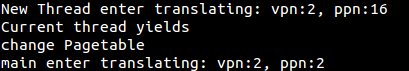
\includegraphics[width=2.5in]{mult.png}
\end{figure}
可见正常切换。

\subsection*{Exercise 6 \& Exercise 7}
这两个练习都是针对缺页处理的,可以一起完成。

lazy-loading有点类似与copy-on-write,在初始化页表的过程中,不确定每一个页表条目对应的物理页号,也不在此时将可执行文件的代码、数据等载入,而是只等到出现 PageFault 时,由对应的处理函数载入对应页面。

在ExceptionHandler中捕获PageFault。捕获之后,如果需要置换页面,就利用页面置换算法找到应该置换的页面。这里需要自行对lazy-loading进行进一步设计,我设计的策略是每个用户程序最多只能占用一定数目的物理页面,同时在替换时只从自己占用的页面中选取,而不干扰别
的用户程序。知道要置换掉哪个页面之后,首先看看页面是否为 dirty ,是的话要写回“磁盘”,也就是写入文件中。然后从文件中读入页面信息,读入内存。

具体实现中,首先需要对AddrSpace类的构造函数进行修改,取消分配物理页号,装载数据段等操作。同时增加创建文件的操作,通过TID标示文件名。
在 TLB miss 处理函数中判断对应表项在 pageTable 中是否为 valid ,
为PageManager新增三个函数载入页面 (loadPage) 、选择置换页面 (getSwapPage) 、置换页面 (swapPage)。并在异常处理程序中加入相应的调用。

具体代码如下:

\begin{lstlisting}
void 
PageManager::loadPage(int address)
{      
     char *filename = currentThread ->space->getFileName();      
     // get the executable file name of the thread
     int phynum;
     int vpn = address/ PageSize;
     printf("PageFault from virtual page %d!\n", vpn);
    
     // find a clean page in the memory for the program     
     int availPage=currentThread->space->getAvailPageNum();
     ASSERT(availPage>=0);
     if(availPage==0) {
         phynum = swapPage();
         ASSERT(phynum!=-1);
     }else{
         phynum = findPage();
         currentThread->space->setAvailPageNum(availPage-1);
         ASSERT(phynum!= -1);
     }
     
     markPage(phynum);     //set the page 
   
     printf("Load virtual page %d to physical page %d from %s\n",
      vpn, phynum, filename);
     
     //open file and load the page
     OpenFile *executable = fileSystem -> Open(filename);
     executable ->ReadAt(&(machine ->mainMemory[phynum * PageSize]),
      PageSize, vpn * PageSize);

     // set the pagetable
     machine ->pageTable[vpn].valid = TRUE;
     machine ->pageTable[vpn].physicalPage = phynum;
     machine ->pageTable[vpn].virtualPage = vpn;
     machine ->pageTable[vpn].use = FALSE;
     machine ->pageTable[vpn].dirty = FALSE;
     machine ->pageTable[vpn].readOnly = FALSE;
     machine->pageTable[vpn].comingTime=stats->totalTicks;

     DumpState();
     delete executable;
}


int
PageManager::swapPage()
{
     int  entryid, phynum, vpn, pagenum;
     pagenum = machine->pageTableSize;
     //entryid= getSwapPageFIFO();  
     entryid = getSwapPageLRU();  
     ASSERT(entryid != -1 && machine->pageTable[entryid].valid==TRUE);

     vpn=machine->pageTable[entryid].virtualPage;
     phynum=machine->pageTable[entryid].physicalPage;
    
    printf("Page Table is full! Page %d will be swapped out!\n",phynum);
     machine ->pageTable[entryid].valid = FALSE;   
     //open file and write memory data, if the page is dirty
     if(machine ->pageTable[entryid].dirty == TRUE)
     {
        char *filename=currentThread->space->getFileName();
        printf("Page %d is dirty, write back to %s\n",phynum, filename);
        
         OpenFile *executable = fileSystem -> Open(filename);     
         executable ->WriteAt(&(machine ->mainMemory[phynum * PageSize]), 
         PageSize, vpn * PageSize);
         delete executable;
     }
     //clean the page
     cleanPage(phynum);  
     return phynum;
}

int
PageManager::getSwapPageFIFO()
{
    DEBUG('a',"PageFault, use FIFO swap\n");
    int slot=0;
    int min = stats->totalTicks;
    int pagenum=machine->pageTableSize;
    for(int i = 0; i< pagenum;i++){     				    
       if(machine->pageTable[i].valid==TRUE &&  
       machine->pageTable[i].comingTime < min){
	   min = machine->pageTable[i].comingTime;
	   slot = i;
	 }
    }
    return slot;
}

int
PageManager::getSwapPageLRU()
{
    DEBUG('a',"PageFault, use LRU swap\n");
    int slot=0;
    int min = stats->totalTicks;
    int pagenum=machine->pageTableSize;
    for(int i = 0; i< pagenum;i++){     				    
       if(machine->pageTable[i].valid==TRUE &&  
       machine->pageTable[i].lastAccessTime < min){
	   min = machine->pageTable[i].lastAccessTime;
	   slot = i;
	 }
    }
    return slot;
}

\end{lstlisting}
在异常处理程序中添加


\begin{lstlisting}
    }else if(which==PageFaultException){
        (stats->numPageFaults) ++;
        int address=machine->registers[BadVAddrReg];
        pageManager->loadPage(address);
	};
\end{lstlisting}
这里的测试比较复杂,我把调试信息打到了文件中,我们可以从文件中判断是否lazy-loading正确。

下面两张图分别是程序一开始的页表状态和中间段的页表状态,我们发现一上来都是PageFault,属于正常的lazy-loading情况。到了中间,当程序缺页的时候,会从替换页面写到文件。测试情况符合逻辑。
\begin{figure}[h!]
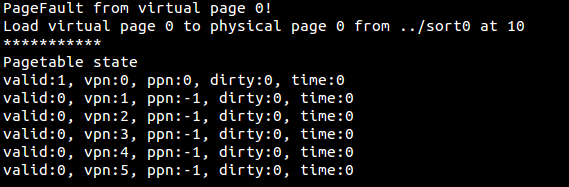
\includegraphics[width=2.5in]{f1.png}
\end{figure}
\begin{figure}[h!]
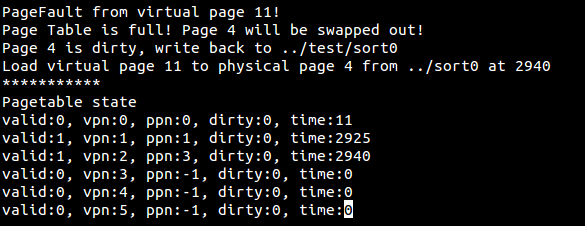
\includegraphics[width=2.5in]{f2.png}
\end{figure}

\section{遇到的困难以及解决办法}
\subsection*{Makefile的修改}
虽然助教在第一节课上讲过怎么样添加一个自己的C文件,这次在实现PageManager上,我尝试过把PageManager单独写成一个cc文件,然后修改Makefile,不过其中的依赖关系实在比较复杂,我一直没有成功编译。最后我采用了投机的办法,把PagaManager类和它的实现都加入了machine.h和machine.cc,从而不用修改Makefile就能够通过编译。
\subsection*{调试}
这次的Lab内容比较多,所以各种错误也比较多,尤其是牵涉到用户程序和内存管理,需要一步一步慢慢地分析。在调试方面我也花了很多时间。

\section{收获与感想}

这次的Lab内容比较多,而且都是实实在在的内容,不花时间是不行的。作为大四学生,我还需要重温两年前学习的操作系统的很多细节内容,也是挺花时间的。也导致了我没有做Challenge了,也是一个遗憾的地方。

当然,这次Lab也让我们进一步理解了操作系统虚拟内存管理上的很多东西,其实Nachos在虚拟内存上的控制已经算比较简单的了,真实的系统中十分复杂。当然,其实这次Lab也对我的毕业设计有一点帮助的地方。在我毕业设计中,我需要为fork()系统调用设计一个文件级别的copy-on-write,这个和本次实验的lazy-loading有一点类似之处,当然我还没有开始设计我的工具,但多少也可以给我一点启发。

\section{意见与建议}
无。

\section{参考资料}
\begin{itemize}
\item 《现代操作系统》
\end{itemize}

\end{document}